\section{Parameter estimation for multi-fidelity Monte Carlo}\label{sec:Parameter_Estimation}

To estimate the correlation coefficients from a pilot sample of size $Q$, we use unbiased Monte Carlo estimators for the sample covariance and standard deviations of the high- and low-fidelity models. Let $\widehat{\text{Cov}}$ denote the sample covariance between the high- and low-fidelity outputs, and let $\widehat\sigma_1$ and $\widehat\sigma_k$ denote their respective sample standard deviations. The resulting estimator for the correlation coefficient is given by
%
\[
\widehat\rho_{1,k} = \frac{\widehat{\text{Cov}}}{\widehat\sigma_1 \widehat\sigma_k} = \frac{\sum_{i=1}^Q\left\langle u_{h,1}^{(i)} - \overline{u}_{h,1},  u_{h,k}^{(i)} - \overline{u}_{h,k} \right\rangle}{\sqrt{\sum_{i=1}^Q \left\langle u_{h,1}^{(i)} - \overline{u}_{h,1}, u_{h,1}^{(i)} - \overline{u}_{h,1} \right\rangle} \sqrt{\sum_{i=1}^Q \left\langle u_{h,k}^{(i)} - \overline{ u}_{h,k}, u_{h,k}^{(i)} - \overline{u}_{h,k} \right\rangle}},
\]
%
where the sample means are defined as $\overline{u}_{h,1} = Q^{-1}\sum_{i=1}^Q u_{h,1}^{(i)}$ and $\overline{  u}_{h,k} = Q^{-1}\sum_{i=1}^Q u_{h,k}^{(i)}$. \JLcolor{Note that the variance estimate is always unbiased. However, for the correlation coefficients, since this estimator involves a non-linear ratio of random variables, it is biased in finite samples and requires large sample size to reduce the bias and achieve consistency with the true population correlation.} To characterize its behavior, we analyze the mean squared error between the true correlation $\rho_{1,k}$ and its sample estimate, decomposed into squared bias and variance
%
\begin{equation}
\label{eq:MSE_rho}
    \mathbb{E}\left[\left(\rho_{1,k} - \widehat\rho_{1,k}\right)^2\right]= \underbrace{\left(\rho_{1,k} - \mathbb{E}\left[\widehat\rho_{1,k}\right]\right)^2}_{\text{Bias}}+\underbrace{\mathbb{E}\left[\left( \mathbb{E}\left[\widehat\rho_{1,k}\right]-\widehat\rho_{1,k}\right)^2\right]}_{\text{Variance}}=\left(\rho_{1,k} - \mathbb{E}\left[\widehat\rho_{1,k}\right]\right)^2+\mathbb{V}\left[\widehat\rho_{1,k}\right].
\end{equation}
%

\subsection{Asymptotic approximations}
To derive asymptotic approximations for the bias and variance, we apply the multivariate delta method \cite{Cr:1946,Oe:1992}, which linearizes a function of random variables via Taylor expansion around its mean. Let the parameter vector be $s = (\rho_{1,k}\sigma_1\sigma_k, \sigma_1, \sigma_k)^T$, and let the sample estimate be $\widehat s = (\widehat{\text{Cov}}, \widehat\sigma_1, \widehat\sigma_k)^T$. Under the central limit theorem, $\widehat s$ converges in distribution to $s$ with $\sqrt{Q}(\widehat s-s)\sim \mathcal{N}(0,\Sigma)$, where $\Sigma$ is the asymptotic covariance matrix of the estimators. Defining the correlation coefficient function $f(s) = s_1 / (s_2 s_3)$, and assuming that the gradient of $f$ exists and is non-zero, we expand $f(\widehat s)$ about $s$ to obtain
%
\begin{equation}
\label{eq:Correlated_Coeff_approx}
  \widehat\rho_{1,k} \approx \rho_{1,k} + \nabla f |_{s}^T \left(\widehat s-s\right), 
  % + \left(s^{(Q)}-s\right)^T H\left(s^{(Q)}-s\right),
\end{equation}
%
where the gradient is $\nabla f|_{s} = (\frac{1}{\sigma_1\sigma_k},-\frac{\rho_{1,k}}{\sigma_1},-\frac{\rho_{1,k}}{\sigma_k} )^T$ and $H$ is the Hessian matrix of the second derivatives. Provided that the components of $\widehat s$ have sufficiently many bounded moments, this expansion gives a valid leading-order approximation of the bias and variance of $\widehat \rho_{1,k}$. In general, for a large sample size $Q (\ge 500)$,  the bias and variance of the sample estimate admit asymptotic expansions of the form
%
\begin{equation*}
\label{eq:Expectation_var_rho}
    \mathbb{E}\left(\widehat \rho_{1,k}\right) =\rho_{1,k}+\frac{a_1}{Q} + \mathcal{O}\left(\frac 1 {Q^2}\right),\qquad \text{Var}\left(\widehat \rho_{1,k}\right)= \frac{a_2}{Q} + \mathcal{O}\left(\frac{1}{Q^2}\right).
\end{equation*}
%
where the constants $a_1$ and $a_2$ depend on the distribution of the underlying random variables. Under the classical assumption of bivariate normality, explicit expressions for these constants are available \cite{Fi:1915, Ha:2007, Ri:1932, So:1913}: $a_1 = -(\rho_{1,k} - \rho_{1,k}^3)/2$ and $a_2 = (1 - \rho_{1,k}^2)^2$. The variance is `instable' since it depends on $\rho_{1,k}$. Using it to construct confidence interval will suffers from the issue that the coverage is not accurate enough. Moreover, the sampling distribution of Pearson's correlation coefficient is not normally distributed. It can be highly skewed, especially when the sample size is small or when the population correlation is near $\pm 1$. This skewed distribution makes it difficult to calculate confidence intervals and conduct statistical tests. In such cases, Fisher's $z$-transformation \cite{Fi:1915, Fi:1921} for $\widehat \rho_{1,k}$ provides an effective means to construct confidence intervals for $\rho_{1,k}$. It shifts $\widehat\rho_{1,k}$ to $\widehat z_k$ via an inverse hyperbolic tangent function
%
\begin{equation}
\label{eq:Fisher_z}
    \widehat z_k  = \text{tanh}^{-1}\left(\widehat\rho_{1,k}\right) = \frac 1 2\ln \left(\frac{1+\widehat\rho_{1,k}}{1-\widehat\rho_{1,k}}\right).
\end{equation}
%
The transformed distribution for $\widehat \rho_{1,k}$ transform correlation coefficients $\widehat \rho_k$ into a variable $\widehat z_k$ that is approximately normally distributed, and the variance ($\text{Var}[\widehat z_k] = 1/(Q - 3)$) is stable in the sense that it is independent of $\rho_{1,k}$. This indicates $\widehat z_k$ is approximately normally distributed even for moderate $Q$. Although its derivation assumes bivariate normality, the transformation remains effective in practice when the data exhibit moderate deviations from normality and are not contaminated by extreme outliers. 

In contrast, our setting does not assume a specific distribution for the model outputs. The bivariate normality assumption is often inappropriate for multifidelity models, where nonlinear mappings or discretization artifacts may induce non-Gaussian dependencies. Instead, a nonparametric asymptotic framework \cite{Og:2006, Pi:1937} is adopted to provide consistent estimators in the large-$Q$ limit ($\ge 500$) without requiring distributional assumptions. In this regime, the leading-order terms simplify to $a_1 = 0$ and $a_2 = 1$. While this asymptotic characterization offers valuable insight, our goal is to design procedures that remain effective for small pilot sample sizes, where these approximations may no longer hold. In particular, the asymptotic expressions for bias and variance cannot reliably inform the choice of $Q$ in practical settings. To address this, we adopt a sequential analysis framework \cite{La:2001,Wa:1947}, which enables dynamic adjustment of the sample size during data collection. Rather than fixing large $Q$ in advance, this approach allows sampling to terminate early once predefined accuracy criteria are satisfied -- offering substantial computational savings over static designs. 


To develop effective stopping rules for this adaptive scheme, we begin by constructing confidence intervals for $\rho_{1,k}$ that remain valid under non-Gaussian output distributions. Additionally, we analyze the sensitivity of the MFMC estimator’s cost-efficiency with respect to perturbations in the estimated correlation coefficient. By combining sensitivity-based diagnostics with confidence interval-based uncertainty quantification, we formulate a robust, real-time adaptive sampling strategy that guarantees accurate correlation estimation and improves the overall effectiveness of the MFMC procedure.

\subsection{Confidence interval for correlation coefficient}
While the dynamic strategy based on cost efficiency and variance reduction is effective, it may terminate prematurely -- before the correlation coefficients are estimated with sufficient accuracy. To mitigate this risk, we introduce an additional stopping criterion based on confidence intervals. Since we do not assume the underlying random variables are normally distributed and aim to work with small pilot sample sizes, nonparametric methods provide a natural solution. In particular, bootstrap techniques \cite{Ef:1979, EfTi:1993} and their extensions \cite{BeDeToMeBaRo:2007} enable the construction of distribution-free confidence intervals through repeated resampling with replacement. These methods are especially effective for small sample sizes (e.g., $Q \leq 30$), requiring minimal assumptions and accommodating non-Gaussian behavior.

When the pilot sample size $Q$ is small and the true correlation is near $\pm 1$, the sampling distribution of the Pearson correlation coefficient becomes notably skewed. To address this issue, we apply the Fisher $z$-transformation to the sample correlation $\widehat \rho_{1,k}$. To further accommodate non-Gaussian behavior, we preprocess the data by ranking the values of $u_{h,1}^{(i)}$ and ${u}_{h,k}^{(i)}$ in {\it ascending order}, and compute the Spearman rank-order correlation coefficient as the Pearson correlation between the ranked values. Applying the Fisher transformation to this rank-based statistic yields a transformed variable $\widehat z_k$ with standard error 
%
\begin{equation}\label{eq:SD_Fisher_Trans}
    \sigma_{\widehat z_k} = 1.03/\sqrt{Q - 3},
\end{equation}
%
as established in \cite{BiHi:2017, FiHaPe:1957}. A $(1 - \alpha)$ confidence interval for $\widehat z_k$ is given by $\widehat z_k \pm z_{\alpha/2}\sigma_{\widehat z_k}$, where the z-score $z_{\alpha/2}$ is the $\alpha/2$-th quantile for the normal distribution. For instance, a $95\%$ confidence interval corresponds to $z_{\alpha/2} = 1.96$. Inverting the Fisher transformation gives the confidence interval for the correlation coefficient $\rho_{1,k}$
%
\begin{align}
    \label{eq:Confidence_Interval_rho}
    \text{CI}_{\rho_{1,k}} &:= \text{tanh}\left(\widehat z_k \pm  z_{\alpha/2}\sigma_{\widehat z_k}\right)
    =\left[1-\frac{2}{\left(\frac{1+\widehat\rho_{1,k}}{1-\widehat\rho_{1,k}}\right)e^{-2z_{\alpha/2}\sigma_{\widehat z_k}}+1}, 1-\frac{2}{\left(\frac{1+\widehat\rho_{1,k}}{1-\widehat\rho_{1,k}}\right)e^{2z_{\alpha/2}\sigma_{\widehat z_k}}+1}\right].
    % = \left[\frac{e^{2(z_k - 1.96\sigma_{z_k})}-1}{e^{2(z_k - 1.96\sigma_{z_k})}+1},\; \frac{e^{2(z_k + 1.96\sigma_{z_k})}-1}{e^{2(z_k + 1.96\sigma_{z_k})}+1}\right].
\end{align}
%
The center and length of the interval can be computed explicitly. The interval length is
%
\[
\text{length} = \frac{2}{\left(\frac{1+\widehat\rho_{1,k}}{1-\widehat\rho_{1,k}}\right)e^{-2z_\alpha\sigma_{\widehat z_k}}+1}-\frac{2}{\left(\frac{1+\widehat\rho_{1,k}}{1-\widehat\rho_{1,k}}\right)e^{2z_\alpha\sigma_{\widehat z_k}}+1}.
\]
%
This expression reveals several key properties. As $\widehat \rho_{1,k}$ increases from $-1$ to $1$, the quantity $\left(\frac{1 + \widehat \rho_{1,k}}{1 - \widehat \rho_{1,k}}\right)$ increases from $0$ to $\infty$. Consequently, both endpoints of the interval increase, resulting in a confidence interval whose center also increases with $\widehat \rho_{1,k}$. When $\widehat \rho_{1,k} \in [0,1]$, the interval length decreases with increasing $\widehat \rho_{1,k}$, and the center of the confidence interval is greater than $\widehat \rho_{1,k}$. When $\widehat \rho_{1,k} \in [-1,0]$, the interval length increases with increasing $\widehat \rho_{1,k}$, and the center is smaller than $\widehat \rho_{1,k}$. The maximum length of the confidence interval occurs at $\widehat \rho_{1,k} = 0$ and is  $2(e^{2z_{\alpha/2}\sigma_{\widehat z_k}}-1)/(e^{2z_{\alpha/2}\sigma_{\widehat z_k}}+1)$. The interval length is an even function of $\widehat \rho_{1,k}$, i.e. length$(\widehat \rho_{1,k})=$ length$(-\widehat \rho_{1,k})$. These properties are illustrated in Figure~\ref{fig:CI_plot}.

If the length of the confidence interval for $\rho_{1,k}$ is denoted by $t_k$, then since the interval is always contained within $[-1, 1]$, we must have $t_k \in (0, 2)$. Let us define the Fisher-transformed scale parameter
\[
A_k := \frac{1 + \widehat \rho_{1,k}}{1 - \widehat \rho_{1,k}},
\]
which satisfies $A_k \in (0, \infty)$ for $\widehat \rho_{1,k} \in (-1, 1)$. Then the quantity
\[
m := e^{2 z_{\alpha/2} \sigma_{\widehat z_k}},
\]
appearing in the confidence interval expression~\eqref{eq:Confidence_Interval_rho}, can be recovered in terms of $t_k$ and $A_k$ as
\[
m = \frac{(A_k^2 + 1) t_k + \sqrt{(A_k^2 - 1)^2 t_k^2 + 16 A_k^2}}{2 A_k (2 - t_k)}.
\]
Using this expression, we obtain an estimate for the required pilot sample size $Q$ needed to achieve a desired confidence interval length $t_k$
\[
Q = 3 + \left( \frac{1.03 \cdot 2 z_{\alpha/2}}{\log m} \right)^2.
\]
This relationship provides a direct link between the accuracy of the correlation estimate (as captured by $t_k$) and the minimum number of samples required to attain that accuracy with high confidence. It is particularly useful for designing adaptive sampling strategies that explicitly control estimation uncertainty through confidence interval widths.


% If the length of the confidence intervals are given as $t_k$, since the confidence interval is always contained within $[-1,1]$, then $t_k\in (0,2)$. Let $A_k = \frac{1 + \widehat \rho_{1,k}}{1 - \widehat \rho_{1,k}}$, then the pilot sample size $Q$ can be estimated as
% \[
% m = e^{2z_{\alpha/2}\sigma_{\widehat z_k}} = \frac{(A_k^2+1)t_k+\sqrt{(A_k^2-1)^2t_k^2+16A_k^2}}{2A_k(2-t_k)}, \quad Q = 3+\left(\frac{1.03\cdot 2z_{\alpha/2}}{\text{ln}(m)}\right)^2.
% \]

%
\begin{figure}[!b]\centering
\begin{tabular}{ccc}
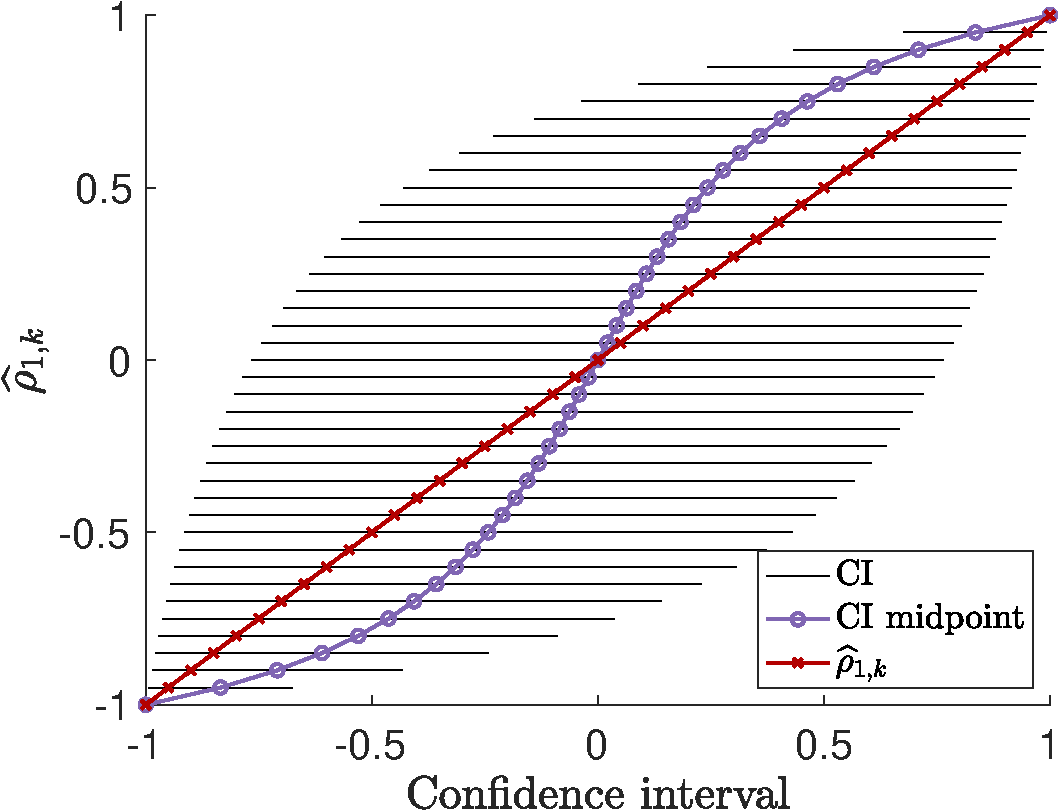
\includegraphics[width=0.3\linewidth]{./figures/CI_Q_5.pdf}&
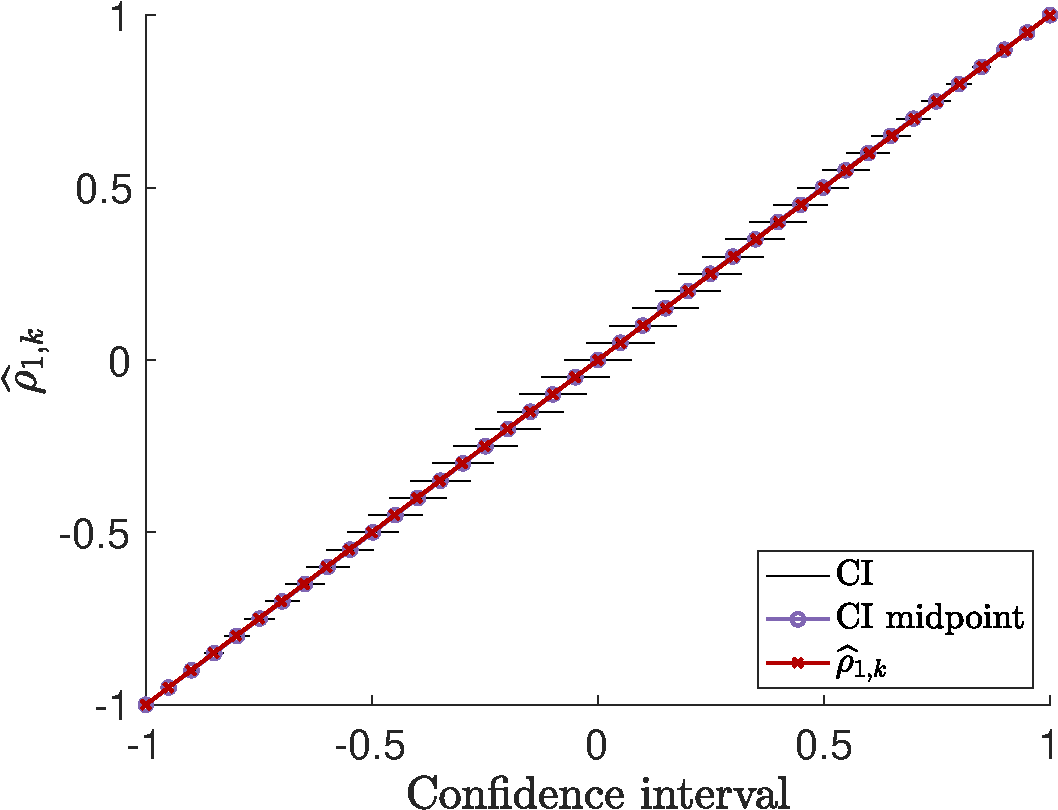
\includegraphics[width=0.3\linewidth]{./figures/CI_Q_30.pdf}&
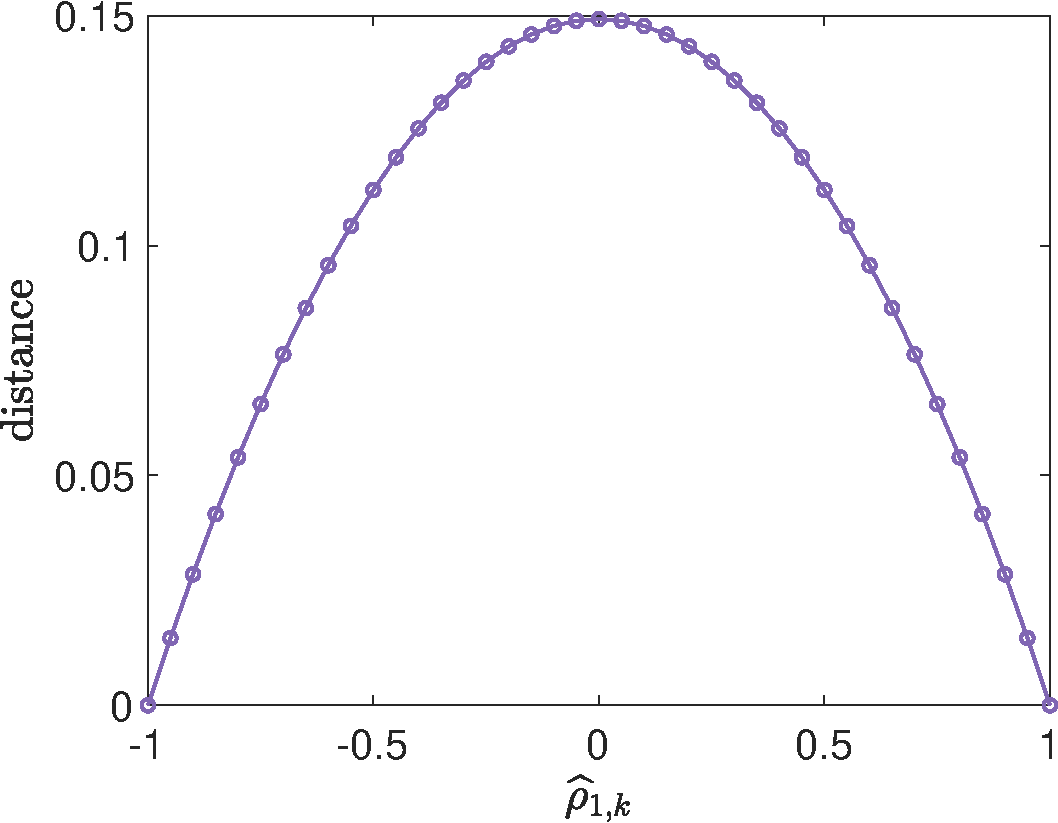
\includegraphics[width=0.3\linewidth]{./figures/CI_distance.pdf}
\end{tabular}
\caption{Left: confidence interval for $\rho_{1,k}$ with $Q=5$. Middle: confidence interval for $\rho_{1,k}$ with $Q=30$. Right: length of confidence interval for $Q=30$. It is an even function in terms of $\widehat \rho_{1,k}$. All plots are generated with $\widehat \rho_{1,k}=-1+0.05t$ with $t=0,\ldots,40$. 95\% confidence interval with $z_{\alpha/2}=1.96$.} 
\label{fig:CI_plot} 
\end{figure}
%


%
\begin{algorithm}[!ht]
\DontPrintSemicolon

    \KwIn{Tolerance $\delta$, splitting ratio $\theta_1 = 0.5$, number of low-fidelity model $K$, initial sample size $Q_0$, sample size correction $dQ = Q_0$. Initializations for Welford's algorithm: proxies of mean, variance and covariance of high- and low-fidelity models $\widehat m_1^{(0)} = 0, \widehat m_k^{(0)} = 0$, $\widehat v_1^{(0)}=0, \widehat v_k^{(0)}=0$, $\widehat r_k^{(0)}=0$.}
    \KwOut{Sample size $Q$ for dynamic sampling, estimated parameters $\sigma_1,\alpha_k, \boldsymbol{\rho}$, cost efficiency $\xi$.}

    
    $\text{AddSample = True}.$

    $p=0, \xi^{(p)} = 0.$
    
    \While{AddSample = True}{
    
    \For{$k=2,\ldots, K$}{
    
        \For{$i = 1,\cdots, dQ $}
    {
    $j=p+i$.
    
    Estimate sample means $\widehat m_1^{(j)}, \widehat m_k^{(j)}$, standard deviations $\widehat\sigma_1^{(j)}, \widehat\sigma_k^{(j)}$, covariances $\widehat{\text{Cov}}^{(j)}$ and correlated coefficients $\widehat\rho_{1,k}^{(j)}$ by Welford's algorithm.
    }
    }
    % [$\text{index},\xi^{(p)}$] = Multi-fidelity Model Selection ($\boldsymbol{\rho}^{(p)},\boldsymbol{C}$).
    
    
    [$\text{index},\xi^{(p+dQ)}$] = Multi-fidelity Model Selection ($\widehat{\boldsymbol{\rho}}^{(p+dQ)},\boldsymbol{C}$).

    

    % Using selected models, estimate pilot sample size $Q_t$ via \eqref{eq:Offline_Sample_Size}.
    
    % Compute  $\xi^{(j)}$ by \eqref{eq:MFMC_sampling_cost_efficiency} with the selected $K^*$ models.
    
    
    \If{$\left|\frac{\xi^{(p+dQ)}-\xi^{(p)}}{\xi^{(p+dQ)}}\right|<\delta$}
    % $\&$ $\left|\frac{\sigma_{k}^{(j)}-\sigma_{k}^{(j-1)}}{\sigma_{k}^{(j)}}\right|<\delta$ $\&$ $\left|\frac{\widehat \sigma_{k}^{(j)}-\widehat \sigma_{k}^{(j-1)}}{\widehat \sigma_{k}^{(j)}}\right|<\delta$ for all $k=2,\ldots, K$}
    {

    Using \eqref{eq:delta_xi_bound} to compute threshold $\delta_1 = 2\delta/(A \sqrt{K^* - 1})$ for $\boldsymbol{\rho}$.
    
    Compute $z_k$ and the confidence interval $\text{CI}_{\rho_{1,k}}$ as in \eqref{eq:Fisher_z} and \eqref{eq:Confidence_Interval_rho}.
    

    
    \If{ the length of confidence interval is bigger than $\delta_1$}
    {
    \text{AddSample = False.}
    }
    \Else {
    \text{AddSample = True.}
    }
    }
    \Else {
    \text{AddSample = True.}
    
    $\xi^{(p)} = \xi^{(p+dQ)}$.
    
     $p=p+dQ$.}
    
    % \If{$j<Q_t$}
    % {
    % AddSample = True
    % }
    
    }    
    
    $Q=j$, $\sigma_1 = \widehat\sigma_1^{(j)}(\text{index})$, $\sigma_k = \widehat\sigma_k^{(j)}(\text{index})$, $\boldsymbol{\rho} = \widehat{\boldsymbol{\rho}}^{(j)}(\text{index})$.
\caption{Dynamic strategy for parameter estimation}\label{algo:Parameter_Estimation}
\end{algorithm}


\subsection{Sensitivity analysis of cost efficiency and variance}
Note that although the correlation coefficients $\rho_{1,k}$ may vary, the sample sizes $N_k^*$ as defined in \eqref{eq:MFMC_SampleSize} are functions of $\rho_{1,k}$ and adjust accordingly. As a result, the variance $\mathbb{V}\left[A^{\text{MF}}\right]$ remains fixed at the target threshold $\epsilon_{\text{tar}}^2$. This implies that $\mathbb{V}\left[A^{\text{MF}}\right]$ is independent of $\rho_{1,k}$, and therefore constant with respect to variations in the correlation coefficients. Consequently, in the sensitivity analysis, it suffices to focus on the cost efficiency $\xi$ as a function of $\rho_{1,k}$.

To analyze the sensitivity of $\xi$ with respect to the correlation coefficients, let $\boldsymbol{\rho}$ denote the true correlation vector, and consider a perturbation $\boldsymbol{\rho} + \Delta \boldsymbol{\rho}$. A first-order Taylor expansion yields the approximation

% Using these two estimates, we determine the optimal choice of $Q$ by ensuring that the mean square error does not exceed a prescribed threshold $\delta$, we allocate a fraction $\theta_1$ to bias and $1-\theta_1$ to variance. Using the error splitting in \eqref{eq:MSE_rho}, we obtain the required pilot sample size
% applying Chebyshev’s inequality $P(|\mathbb{E}(\rho_{1,k}^{(Q)})-\rho_{1,k}^{(Q)}|\ge \nu)\le \text{Var}(\rho_{1,k}^{(Q)})/\nu^2$ with $\nu = (1-\theta_1)\delta_1$ gives
% %
% \[
% P\left(\left|\mathbb{E}\left(\rho_{1,k}^{(Q)}\right)-\rho_{1,k}^{(Q)}\right|\ge \nu\right)\le \frac{\text{Var}\left(\rho_{1,k}^{(Q)}\right)}{\nu^2}
% \]
% %
% %
% \[
% \frac{(1-\rho_{1,k}^2)^2}{Q\nu^2} = \frac{(1-\rho_{1,k}^2)^2}{(1-\theta_1)^2Q\delta_1^2}\le 1\rightarrow Q\ge \frac{(1-\rho_{1,k}^2)^2}{(1-\theta_1)^2\delta_1^2}.
% \]
% %
% Combining these results, a lower bound on $Q$ can be determined as
%
% \begin{equation}
% \label{eq:Offline_Sample_Size}
%     Q\ge \max_{k} \left(\frac{\left|a_1\right|}{\sqrt{\theta_1\delta} }, \frac{a_2}{(1-\theta_1)\delta}\right).
% \end{equation}
% %
% Note in \eqref{eq:Offline_Sample_Size}, we still need to estimate the true correlation coefficients in order to estimate the lower bound of pilot sample size $Q$. However, the sample statistics also depends on $Q$,  we thus  iteratively update $Q$ until convergence is reached. % However, when sampling with a small sample size that does not rely on assumptions about the underlying data distribution, non-parametric method like  bootstrapping \cite{Wa:2006} and sequential analysis \cite{Wa:1947} provide alternative strategies for estimating $Q$. 



%
\[
\Delta\xi=\xi(\boldsymbol{\rho}+\Delta \boldsymbol{\rho}) - \xi(\boldsymbol{\rho}) \approx \sum_{k=2}^K \frac{\partial \xi}{\partial \rho_{1,k}} \Delta\rho_{1,k},
% \quad \quad \Delta \mathbb{V}\left[A^{\text{MF}}\right]\approx \sum_{k=2}^K \frac{\partial  \mathbb{V}\left[A^{\text{MF}}\right]}{\partial  \rho_{1,k}}  \Delta\rho_{1,k},
\]
%
where the partial derivatives quantify the sensitivities of $\xi$  to perturbations in the correlation coefficients. The partial derivatives of $\xi$ to perturbations in the correlation coefficients are
%
\begin{align}
% \frac{\partial  \xi}{\partial  \rho_{1,1}} &=\frac{2\sum_{j=1}^K\sqrt{C_j\left(\rho_{1,j}^2 - \rho_{1,j+1}^2\right)}}{C_1}\frac{C_1\rho_{1,1}}{\sqrt{C_1(\rho_{1,1}^2-\rho_{1,2}^2)  }}\\
\label{eq:partial_xi_rho}
\frac{\partial  \xi}{\partial  \rho_{1,k}} 
&=\frac{2SS^\prime}{C_1}, \quad \forall\; k=2,\ldots, K,
% \label{eq:partial_var_rho}
% \frac{\partial  \mathbb{V}\left[A^{\text{MF}}\right]}{\partial  \rho_{1,k}} 
% &=2\sigma_1^2\rho_{1,k}\left(\frac{1}{N_{k}} - \frac{1}{N_{k-1}}\right)-\left( \frac{\Delta_{k-1}}{N_{k-1}^2}\frac{\partial N_{k-1}}{\partial  \rho_{1,k}}+\frac{\Delta_{k} }{N_k^2}\frac{\partial N_k}{\partial  \rho_{1,k}}\right)=\epsilon_{\text{tar}}^2\frac{S^\prime \left(S-T\right)}{S^2},
\end{align}
%
with
%
\begin{align}
\label{eq:S_n_S_prime}
S& = \sum_{j=1}^K\sqrt{C_j\left(\rho_{1,j}^2-\rho_{1,j+1}^2\right)},\quad
S^\prime = \frac{\partial  S}{\partial  \rho_{1,k}} = \rho_{1,k}\left(\sqrt{\frac{C_k}{\rho_{1,k}^2-\rho_{1,k+1}^2}} - \sqrt{\frac{C_{k-1}}{\rho_{1,k-1}^2-\rho_{1,k}^2}}\right),\\
% \nonumber
% T &=  \sqrt{C_{k-1}\left(\rho_{1,k-1}^2 - \rho_{1,k}^2\right)} + \sqrt{C_{k}\left(\rho_{1,k}^2 - \rho_{1,k+1}^2\right)} = \frac{1}{\sigma_1}\left[\sqrt{C_{k-1}\Delta_{k-1}} + \sqrt{C_{k}\Delta_{k}}\right],\\
\nonumber
\frac{\partial N_{k}}{\partial  \rho_{1,k}}&=\frac{\sigma_1^2}{\epsilon_{\text{tar}}^2}\left[\frac{\rho_{1,k}}{\sqrt{C_{k}\left(\rho_{1,k}^2 - \rho_{1,k+1}^2\right)}}S+S^\prime \sqrt{\frac{\rho_{1,k}^2 - \rho_{1,k+1}^2}{C_{k}}}\right],\\
% \nonumber
% \frac{\partial N_{k-1}}{\partial  \rho_{1,k}}&=\frac{\sigma_1^2}{\epsilon_{\text{tar}}^2}\left[\frac{-\rho_{1,k}}{\sqrt{C_{k-1}\left(\rho_{1,k-1}^2 - \rho_{1,k}^2\right)}}S+S^\prime \sqrt{\frac{\rho_{1,k-1}^2 - \rho_{1,k}^2}{C_{k-1}}}\right].
% S^{\prime\prime}&= \frac{\partial^2  S}{\partial^2  \rho_{1,k}} = \frac{S^\prime}{\rho_{1,k}} - \rho_{1,k}^2\left(\frac{\sqrt{C_k}}{(\rho_{1,k}^2-\rho_{1,k+1}^2)^{3/2}}+\frac{\sqrt{C_{k-1}}}{(\rho_{1,k-1}^2-\rho_{1,k}^2)^{3/2}}\right).
\end{align}
%



Under standard MFMC assumptions, the derivative $S^\prime$ is negative, while $S$ is always positive. Consequently, the partial derivatives $\partial \xi / \partial \rho_{1,k}$ is negative. This implies that increasing $\rho_{1,k}$ improves cost efficiency and reduces the variance of the estimator. To quantify the impact of correlation errors, we apply the Cauchy–Schwarz inequality to obtain bounds on the relative errors
%
\begin{align}
\label{eq:delta_xi_bound}
    \frac{\left|\Delta \xi\right|}{\xi}&\le \underbrace{\frac{1}{\xi}\sqrt{\sum_{k=2}^K \left(\frac{\partial \xi}{\partial \rho_{1,k}}\right)^2}}_{A_0} \cdot \sqrt{\sum_{k=2}^K\left(\Delta\rho_{1,k}\right)^2}=\frac{2}{S}\sqrt{\sum_{k=2}^K(S^\prime)^2} \cdot \sqrt{\sum_{k=2}^K\left(\Delta\rho_{1,k}\right)^2},
    % \label{eq:delta_var_bound}
    % \frac{\left|\Delta \mathbb{V}\left[A^{\text{MF}}\right]\right|}{\mathbb{V}\left[A^{\text{MF}}\right]}&\le
    % % \le \underbrace{\frac{1}{\mathbb{V}\left(A^{\text{MF}}\right)}\sqrt{\sum_{k=2}^K \left(\frac{\partial \mathbb{V}\left(A^{\text{MF}}\right)}{\partial \rho_{1,k}}\right)^2}}_{A_1}\cdot \sqrt{\sum_{k=2}^K\left(\Delta\rho_{1,k}\right)^2}=
    % \underbrace{\frac{1}{S^2}\sqrt{\sum_{k=2}^K\left(S^\prime \left(S-T\right)\right)^2}}_{A_1}\cdot \sqrt{\sum_{k=2}^K\left(\Delta\rho_{1,k}\right)^2}.
\end{align}
%
To enforce accuracy in the correlation estimates, we introduce a user-defined relative tolerance $\delta$ and impose the bound $|\Delta \rho_{1,k}| \le \delta / (A_0 \sqrt{K - 1})$ ensures that the total relative errors in both cost efficiency and variance remain below $\delta$.




% \JLcolor{Given $\delta$, we first estimate $C^\prime$, then choose $\delta_2$ as $\delta/C^\prime$, $\delta_1=\delta_2/\sqrt{K-1}$, and select $N$ by \eqref{eq:Offline_Sample_Size} for all $k$.}


% The term $\left(1-\sqrt{\frac{C_{k-1}(\rho_{1,k}^2-\rho_{1,k+1}^2)}{C_k(\rho_{1,k-1}^2-\rho_{1,k}^2)}}\right)$ in $\partial \xi/\partial \rho_{1,k}$ encodes MFMC’s selection criteria, ensuring the derivative’s negativity when models are optimally ordered. This indicates that higher $\rho_{1,k}$ improves low-fidelity models’ variance reduction efficiency, reducing reliance on costly high-fidelity evaluations. This reinforces the idea that high-quality low-fidelity models—those that are more aligned with the high-fidelity results—can significantly lower the reliance on expensive high-fidelity evaluations, making the entire multi-fidelity approach more cost-effective.



\section{Model selection for Multi-fidelity Monte Carlo}\label{sec:Model_Selection}
After constructing the confidence intervals \eqref{eq:Confidence_Interval_rho} for the estimated correlation coefficients $\{\widehat\rho_{1,k}\}_{k=1}^{K}$ 
associated with a set of $K$ candidate models $\mathcal{S}=\{ u_{h, k}\}_{k=1}^K$, the next step is to identify a subset $\mathcal{S}^* \subseteq \mathcal{S}$ to be used in multifidelity Monte Carlo estimation \cite{PeWiGu:2016}. The selection of $\mathcal{S}^*$ must meet two key criteria. First, the estimated correlation coefficients must satisfy the assumptions of Theorem~\ref{thm:Sample_size_est}, and second, the selected subset should maximize computational efficiency, as quantified by the metric $\xi$.

A key challenge arises when the confidence intervals for the correlation estimates ${\widehat\rho_{1,k}}$ exhibit significant overlap, as shown in Figure~\ref{fig:CI_plot}. In such cases, the close proximity of correlation coefficient estimates may obscure meaningful differences in model quality. Notably, overlapping confidence intervals do not imply statistical equivalence of the underlying correlations, and additional statistical tools are needed to resolve this ambiguity. 

\JLcolor{To address this issue, we use a one-tailed $z$-test to assess if there's a statistically significant difference between the means of two populations based on samples from those populations. The standard version of the test assumes normally distributed variables, which does not hold for sample correlation coefficients in our setting.} To overcome this limitation, we apply the Delta method \cite{BeKo:2023,CaBe:1990,LeCa:1998} to linearize the nonlinear constraints via a first-order Taylor expansion for the transformed variables, which are approximately normally distributed. Then perform the hypothesis testing. \JLcolor{Note that The t-test does not have a minimum sample requirement, the reliability of delta method depends on the central limit theorem, which generally requires a pilot sample size of at least 30. A larger sample size is recommended for more accurate results. For smaller
$Q$, however, the normality assumption may break down, and nonparametric alternatives (e.g., bootstrap tests) may be preferable.}
\newline 

% \noindent {\bf Bootstrap method}
% This method exploits the flexibility of the bootstrap without making distributional assumptions about the correlation estimates, though at the cost of additional sampling. The approach involves generating $B$ bootstrap replicates to construct empirical distributions of relevant statistics. 

% For condition (i) in Theorem~\ref{thm:Sample_size_est}, we test whether there is a statistically significant decrease in correlation coefficients between adjacent models with potential overlap of confidence intervals. Define the null hypothesis $H_0$: $|\rho_{1,k}| \leq |\rho_{1,k+1}|$, and the alternative hypothesis $H_a$: $|\rho_{1,k}| > |\rho_{1,k+1}|$. For each bootstrap replicate $b$, we compute the absolute correlation estimates $|\widehat\rho_{1,k}^{(b)}|$ and $|\widehat\rho_{1,k+1}^{(b)}|$, and construct a $(1-\alpha)$ confidence interval for their differences $|\widehat\rho_{1,k}^{(b)}| - |\widehat\rho_{1,k+1}^{(b)}|$, where $\alpha$ is  significance level. If the lower bound of this interval is positive,  $H_0$ is rejected in favor of $H_a$, indicating a significant drop in correlation. To verify condition (ii) of Theorem~\ref{thm:Sample_size_est}, we evaluate for each replicate the following difference statistic 
% %
% \[
% D_k^{(b)} = C_{k-1}\left[\left(\widehat\rho_{1,k}^{(b)}\right)^2-\left(\widehat \rho_{1,k+1}^{(b)}\right)^2\right]-C_k\left[\left(\widehat\rho_{1,k-1}^{(b)}\right)^2-\left(\widehat \rho_{1,k}^{(b)}\right)^2\right].
% \]
% %
% A $(1 - \alpha)$ confidence interval for $D_k^{(b)}$ is then constructed. If its lower bound is positive, condition (ii) is deemed satisfied.
% \newline 

Let $\mathcal{I} = \{1,\ldots,K\}$ denote the ordered indices corresponding to the models in $\mathcal{S}$, and let $\mathcal{I}^*\subseteq \mathcal{I}$ represent the indices of the selected subset $\mathcal{S}^*$. Since the high-fidelity model $u_{h,1}$ is always included, both $\mathcal{I}$ and $\mathcal{I}^*$ must contain index 1. The objective, then, is to identify an optimal index subset $\mathcal{I}^*$ of size $K^* = |\mathcal{I}^*| \leq K$ such that the resulting model combination minimizes $\xi$ while satisfying the conditions of Theorem~\ref{thm:Sample_size_est}.


\begin{theorem} \label{thm:Model_Selection}
$Q\ge 30$. We first order the models by decreasing $|\widehat \rho_{1,k}|$ for all $k$. Following are the criterion for the three conditions required for model selection, including t statistics and their corresponding degree of freedom. Let $\widehat\lambda_k = 1-\widehat\rho_{1,k}^2$.

\noindent {\bf Condition (i) of Theorem~\ref{thm:Sample_size_est}}
%
\begin{equation}\label{eq:Conidtion_1_t_test}
    t_k =\frac{\widehat \rho_{1,k}^2-\widehat \rho_{1,k+1}^2}{\frac{1.03}{\sqrt{Q-3}}\cdot 2\sqrt{\widehat \rho_{1,k}^2\left(1-\widehat \rho_{1,k}^2\right)^2 +\widehat \rho_{1,k+1}^2\left(1-\widehat \rho_{1,k+1}^2\right)^2}}, 
    % \quad \nu = \left\lfloor(Q-1)\frac{\left(\widehat\lambda_k^2 + \widehat\lambda_{k+1}^2\right)^2}{\widehat\lambda_k^4 + \widehat\lambda_{k+1}^4}\right\rfloor.
\end{equation}
%
\noindent {\bf Condition (ii) of Theorem~\ref{thm:Sample_size_est}}

\begin{align*}
    t_k&= \frac{-C_{k}\widehat\rho_{1,k-1}^2+(C_{k-1} + C_k)\widehat \rho_{1,k}^2  - C_{k-1}\widehat \rho_{1,k+1}^2}{\frac{1.03}{\sqrt{Q-3}}\cdot 2\sqrt{C_k^2\widehat\rho_{1,k-1}^2\widehat\lambda_{k-1}^2+(C_{k-1} + C_k)^2 \widehat\rho_{1,k}^2 \widehat\lambda_k^2+C_{k-1}^2 \widehat\rho_{1,k+1}^2 \widehat\lambda_{k+1}^2}},\\
    &=\frac{C_k \widehat \lambda_{k-1} - (C_{k-1} + C_k)\widehat \lambda_{k} + C_{k-1} \widehat \lambda_{k+1}}{\frac{1.03}{\sqrt{Q-3}}\cdot 2\sqrt{C_k^2 (1-\widehat\lambda_{k-1})\widehat\lambda_{k-1}^2+(C_{k-1} + C_k)^2 (1-\widehat\lambda_k) \widehat\lambda_k^2+C_{k-1}^2 (1-\widehat\lambda_{k+1})\widehat\lambda_{k+1}^2}}
\end{align*}


% \[
% \nu=\left\lfloor(Q-1)\frac{\left(C_{k-1}\left[\widehat \rho_{1,k}^2\widehat\lambda_k^2 +\widehat \rho_{1,k+1}^2\widehat\lambda_{k+1}^2\right] + C_{k}\left[\widehat \rho_{1,k-1}^2\widehat\lambda_{k-1}^2 +\widehat \rho_{1,k}^2 \widehat\lambda_k^2\right]\right)^2 }{C_{k-1}^2 \left[\widehat \rho_{1,k}^2\widehat\lambda_k^2 +\widehat \rho_{1,k+1}^2\widehat\lambda_{k+1}^2\right]^2 + C_{k}^2\left[\widehat \rho_{1,k-1}^2\widehat\lambda_{k-1}^2 +\widehat \rho_{1,k}^2 \widehat\lambda_k^2\right]^2}\right\rfloor
% \]

\noindent {\bf Select the models with smallest sampling cost.}


Define 
\[
\widehat\eta_{i_p} = \widehat\rho_{1,{i_p}} \left(\frac{-\sqrt{C_{i_{p-1}}}}{\sqrt{ \widehat\rho_{1,{i_{p-1}}}^2-\widehat\rho_{1,{i_{p}}}^2}}+\frac{\sqrt{C_{i_p}}}{\sqrt{ \widehat\rho_{1,{i_p}}^2-\widehat\rho_{1,{i_{p+1}}}^2}} \right),
\]

%
\[
t_k = \frac{\sum_{p=1}^{K_1^*}\sqrt{C_{i_p}(\widehat \rho_{1,i_p}^2-\widehat\rho_{1,i_{p+1}}^2)} - \sum_{p=1}^{K_2^*}\sqrt{C_{j_p}(\widehat \rho_{1,j_p}^2-\widehat\rho_{1,j_{p+1}}^2)}}{\frac{1.03}{\sqrt{Q-3}}\sqrt{\sum_{p=1}^{K_1^*} \widehat\lambda_{i_p}^2 \widehat\eta_{i_p}^2 + \sum_{p=1}^{K_2^*} \widehat\lambda_{j_p}^2 \widehat\eta_{j_p} ^2}}, 
\]
%

% %
% \[
% \nu = \left\lfloor (Q-1)\frac{\left[\sum_{p=1}^{K_1^*}\widehat\lambda_{i_p}^2\widehat\eta_{i_p}^2 +\sum_{p=1}^{K_2^*} \widehat\lambda_{j_p}^2 \widehat\eta_{j_p}^2\right]^2}{\left[\sum_{p=1}^{K_1^*}\widehat\lambda_{i_p}^2\widehat\eta_{i_p}^2\right]^2 + \left[\sum_{p=1}^{K_2^*} \widehat\lambda_{j_p}^2 \widehat\eta_{j_p}^2\right]^2}\right\rfloor.
% \]
% %
Starting from index 1, we discard the current model $k+1$ if  the following two conditions does not hold. Then we select the models with the smallest sampling cost, discard the set of models if the total cost is larger.
\end{theorem}




% If sample variances are similar in the sense that $0.5<\sigma_{z_k}^2/\sigma_{z_{k+1}}^2<2$, the corresponding $t$ statistic is
% \[
% t_k=\frac{D}{s_p\sqrt{\frac{1}{Q_1}+\frac{1}{Q_2}}}, \quad s_p = \sqrt{\frac{(Q_1 - 1)\sigma_{z_k}^2 + (Q_2 - 1)\sigma_{z_{k+1}}^2}{Q_1+Q_2-2}}
% \]
% Otherwise,

% \[
% t_k = \frac{\Delta z_k}{\sqrt{\frac{\sigma_{z_k}^2}{Q_1} + \frac{\sigma_{z_{k+1}}^2}{Q_2}}}
% \]



% %
% \begin{equation*}\label{eq:Optimization_pb_model_selection}
%     \begin{array}{lll}
%     \displaystyle\min_{S^*} &\displaystyle \xi,\\
%        \text{s.t.} &\displaystyle |\rho_{1,1}|>\ldots>|\rho_{1,K^*}|,\\
%        &\displaystyle \frac{C_{i-1}}{C_i}>\frac{\rho_{1,i-1}^2-\rho_{1,i}^2}{\rho_{1,i}^2-\rho_{1,i+1}^2}, \quad i=1,\ldots,{K^*}, \quad \rho_{1,K^*+1}=0,\\
%     \end{array}
% \end{equation*}
% %

The confidence interval, [\sout{together with the sensitivity analysis}], forms the basis of a robust stopping rule for adaptive sampling. Specifically, we determine the minimal pilot sample size $Q$ required for reliable parameter estimation by sequentially updating sample statistics as $Q$ increases \cite{La:2001,Wa:1947}. Sampling continues until both accuracy and confidence criteria are satisfied. This adaptive strategy is summarized in Algorithm~\ref{algo:Parameter_Estimation} and is integrated into the enhanced model selection procedure described in Section~\ref{sec:Model_Selection} (Algorithm~\ref{algo:MFMC_Algo_model_selection}).


\normalem
\begin{algorithm}[!ht]
\label{algo:MFMC_Algo_model_selection}
\DontPrintSemicolon    
   \KwIn{$K$ candidate models $u_{h, k}$ with coefficients $\widehat \rho_{1,k}$, $\widehat\sigma_1$, $\widehat\sigma_k$ and cost per sample $C_k$.}\vspace{1ex}
    
    \KwOut{Selected $K^*$ models $ u_{h, i}$ in $\mathcal{S}^*$, with coefficients $\widehat\rho_{1,i}$ and $C_i$ for each model $ u_{h, i}$.}\vspace{1ex}
    \hrule \vspace{1ex}

   % Estimate $\rho_{1,k}$ and $C_k$ for each model $u_{h, k}$ using $N_0$ samples.
   
   
   Sort $u_{h, k}$ by decreasing $|\widehat \rho_{1,k}|$ with t test using the t statistics \eqref{eq:Conidtion_1_t_test} to create $\mathcal{S}=\{u_{h, k}\}_{k=1}^K$. 
   
   Initialize $w^*=C_1$, $\mathcal{S}^*=\{u_{h, 1}\}$. Let $ \mathcal{\widehat S}$ be all $2^{K-1}$ ordered subsets of $\mathcal{S}$, each containing $u_{h, 1}$. 
   % Set $ \mathcal{\widehat S}_1=\mathcal{S}^*$.

    % $(2 \le j \le 2^{K-1})$
    \For{each subset $\mathcal{\widehat S}_j$\,}{

    {
    \If{ condition $(ii)$ from Theorem \ref{thm:Sample_size_est} is satisfied using \eqref{eq:Conidtion_2_t_test}}{
    Compute the objective function value $w$ using \eqref{eq:MFMC_sampling_cost_efficiency}.
    
    \If{Check \eqref{eq:cost_decrease_t_test}}{
    {
    Update $\mathcal{S}^* = \mathcal{\widehat S}_j$ and $w^* = w$.
    }
    } 
    }
    }
    $j=j+1$.
    }
    % Compute $\alpha_i$ for $\mathcal{S}^*$, $i=2,\dots, K^*$ by \eqref{eq:MFMC_coefficients}.
\caption{Multi-fidelity Model Selection}
\end{algorithm}
\ULforem


% \normalem
% \begin{algorithm}[!ht]
% \label{algo:enhanced_mfmc_selection}
% \DontPrintSemicolon
% \SetAlgoVlined
% \SetKwProg{Fn}{Function}{}{}
% \SetKwInOut{Input}{Input}
% \SetKwInOut{Output}{Output}

% \Input{%
% Vectors of correlation coefficients $\boldsymbol{\rho}$, costs per sample $\boldsymbol{C}$, sample deviations $\boldsymbol{\sigma}$. 
% }
% \Output{%
%   Set of selected models $\mathcal{S}^*=\{u_{h,i}\}_{i\in I^*}$, correlations of selected models $\boldsymbol{\rho}^*$, costs of selected models $\boldsymbol{C}^*$, minimal cost efficiency ratio $\xi_{\text{min}}$, weights $\alpha_i^*$.
% }
% \hrule
 
% \Fn{[idx\textunderscore for\textunderscore model, $\xi_{\text{min}}$] = Model\textunderscore Selection\textunderscore Backtrack ($\boldsymbol{\rho}, \boldsymbol{C}$)}{
% Sort the correlation coefficients by non-increasing $|\rho_{1,k}|$ with order $r$. Relabel $\rho_{1,k}, C_k$ for all $k$ as $\boldsymbol{\rho}, \boldsymbol{C}$.


% Initialization: 
% current$\_$idx = 1, $\xi_{\text{min}}=1$, global$\_$idx = []. %$\boldsymbol{\rho}=[1]$, $\boldsymbol{C}=[C_1]$,


% \vspace{3mm}
% \textbf{Backtrack} $(\text{current}\_\text{idx},\, \xi_{\text{min}},\, 2)$. 

% idx\textunderscore for\textunderscore model = r(global$\_$idx).
% \vspace{3mm}

% \Fn{ $[\mathcal{S}^*,\, \boldsymbol{\rho}^*, \,\boldsymbol{C}^*, \xi_{\text{min}}]$ = \textbf{Backtrack} $\left(\text{current}\_\text{idx}, \, \xi, \,k_{\text{next}}\right)$}{


%   \If{$\xi \leq \xi_{\text{min}}\,$ }{
%     $\xi_{\text{min}}=\xi$.

%     global$\_$idx = current$\_$idx.
%   }
%   % \Else {
%   %   $\mathcal{S}^* = \mathcal{S}$, $\boldsymbol{\rho}^* = \boldsymbol{\rho}$, $\boldsymbol{C}^* = \boldsymbol{C}$, $\xi_{\text{min}}=\xi$.
%   % }
  
%   \If{$k_{\text{next}} > K$}{ 
%     \Return
%   }
  
%   \For{$k = k_{\text{next}}$ \textbf{to} $K$}{ 
%      % $\rho_{1,\text{last}} = \boldsymbol{\rho}_{\text{end}}$, $C_{\text{last}} = \boldsymbol{C}_{\text{end}}$.
%      previous\textunderscore idx = current$\_$idx (end).

%      % $\rho_k = \boldsymbol{\rho}(k), C_k = \boldsymbol{C}(k)$

%      % $\rho_{\text{next}}=0$

     
%     \If{% 
%       $\frac{\boldsymbol{C}({\text{previous}\_\text{idx}})}{\boldsymbol{C}(k)} > \frac{\boldsymbol{\rho}({\text{previous}\_\text{idx}})^2 - \boldsymbol{\rho}(k)^2}{\boldsymbol{\rho}(k)^2}$ 
%     }{
%         Continue to next iteration.
%     }

%         % $\rho_k\_$vec = [$\boldsymbol{\rho}$(cur$\_$ind), $\rho_k$]
        
%         Compute $\xi$ via \eqref{eq:MFMC_sampling_cost_efficiency} for indices  
%       [current\textunderscore idx, $k$].

%       \If{$\xi\ge \xi_{\text{min}}$ or $\,\xi>1$}{ 
%     Continue to next iteration.
%     }
      
%       \textbf{Backtrack} $(\, [\text{current}\_\text{idx},k],\xi, k+1)$.
%   }
% }
% }
% \vspace{3mm} 


 
% $I^* = \text{idx}\_\text{for}\_\text{model}, K^* = |I^*|, \boldsymbol{\rho}^* = \boldsymbol{\rho} (I^*)$, $\boldsymbol{C}^* = \boldsymbol{C} (I^*)$, $\boldsymbol{\sigma}^* = \boldsymbol{\sigma} (I^*)$.

% Selected models $\mathcal{S}^* = \{u_{h,k}\}_{k\in \mathcal{I^*}}$ with weights $\alpha_i^*$ for $i=2,...,K^*$ via \eqref{eq:MFMC_SampleSize}.




% \caption{Multi-fidelity Model Selection with Backtracking Pruning}
% \end{algorithm}
% \ULforem




\normalem
\begin{algorithm}[!ht]
\label{algo:MFMC_Algo}
\DontPrintSemicolon

    
   \KwIn{Selected $K^*$ models $u_{h, k}$ in $\mathcal{S}^*$, parameters $\rho_{1,k}$, $\alpha_k$ and $C_k$ for each $u_{h, k}$,  tolerance $\epsilon$. }\vspace{1ex}
    
    \KwOut{Sample sizes $N_k$ for $K^*$ models, expectation 
    estimate $A^{\text{MF}}$.}\vspace{1ex}
    \hrule \vspace{1ex}
    

    Compute the sample size $N_k$ for $1\leq k\leq K^*$ by \eqref{eq:MFMC_SampleSize} and generate i.i.d. $N_1$ and $N_k-N_{k-1}$ samples for $k=2,\ldots, K^*$.

    Evaluate $u_{h, 1}$ to obtain $u_{h, 1}(\boldsymbol{\omega}^i)$ for $i = 1,\ldots,N_1$ and compute $A_{1,N_1}^{\text{MC}}$ by \eqref{eq:MC_estimator}.
    
    \For{$k = 2,\ldots,K^* $\,}{

    Evaluate $u_{h, k}$ to obtain $u_{h, k}(\boldsymbol{\omega}^i)$ for $i = 1,\ldots,N_{k-1}$ and compute $A_{k,N_{k-1}}^{\text{MC}}$ by \eqref{eq:MC_estimator}.

    Evaluate $u_{h, k}$ to obtain $u_{h, k}(\boldsymbol{\omega}^i)$ for $i = 1,\ldots,N_k-N_{k-1}$ and compute $A_{k,N_k\backslash N_{k-1}}^{\text{MC}}$ by \eqref{eq:MC_estimator}.

    % Store $N_{k-1}$ and $N_{k}-N_{k-1}$ samples as $N_k$ samples.
    }

    Compute $A^{\text{MF}}$ by \eqref{eq:MFMC_estimator_independent}.
    
\caption{Multifidelity Monte Carlo}
\end{algorithm}
\ULforem

% \normalem
% \begin{algorithm}[!ht]
% \label{algo:MFMC_Algo}
% \DontPrintSemicolon

    
%    \KwIn{Models $f_k$ in $\mathcal{S}^*$, parameters $\rho_k$, $\alpha_k$ and $C_k$ for each $f_k$ in $\mathcal{S}^*$,  tolerance $\epsilon$. }\vspace{1ex}
    
%     \KwOut{Sample sizes $N_k$ for $K^*$ models, expectation 
%     estimate $A^{\text{MFMC}}$.}\vspace{1ex}
%     \hrule \vspace{1ex}
%     Compute initial sample sizes $\boldsymbol{N}=[N_1,\ldots, N_{K^*}]$ using \eqref{eq:MFMC_SampleSize}. Set $\boldsymbol{N}_{\text{old}} = \boldsymbol{0}$ and $\boldsymbol{dN} = \boldsymbol{N}$. 
    
%     Initialize sample means $A_{1,N_1}^{\text{MC}}, A_{k,N_{k-1}}^{\text{MC}}, A_{k,N_k\backslash N_{k-1}}^{\text{MC}}=0. $
    
%     \While{$\sum_k dN_k>0$\,}{

%     Evaluate $dN_{1}$ samples for $f_1$ to obtain $f_1(\boldsymbol{\omega}^i)$. Update $A_{1,N_1}^{\text{MC}} = \frac{\boldsymbol{N}_{\text{old}}^1 A_{1,N_1}^{\text{MC}}+\sum_i f_1(\boldsymbol{\omega}^i)}{\boldsymbol{N}_{\text{old}}^1+dN_1}$ and $\sigma_1$.

%     Store $dN_1$ samples.
    
%     \For{$2\le k\le K^*$\,}{
    
%         % \For{$i = 1,\ldots,dN_k $\,}
%     % {
%     Evaluate previously stored $dN_{k-1}$ samples for $f_k$ to obtain $f_k(\boldsymbol{\omega}^i)$. Update $A_{k,N_{k-1}}^{\text{MC}} = \frac{\boldsymbol{N}_{\text{old}}^k A_{k,N_{k-1}}^{\text{MC}}+\sum_i f_k(\boldsymbol{\omega}^i)}{\boldsymbol{N}_{\text{old}}^k+dN_{k-1}}$. 
    
%     Collect new $dN_{k}-dN_{k-1}$ samples. Evaluate $f_k$ to obtain $f_k(\boldsymbol{\omega}^i)$. Update $A_{k,N_k\backslash N_{k-1}}^{\text{MC}} = \frac{\boldsymbol{N}_{\text{old}}^k A_{k,N_k\backslash N_{k-1}}^{\text{MC}}+\sum_i f_k(\boldsymbol{\omega}^i)}{\boldsymbol{N}_{\text{old}}^k+dN_{k}-dN_{k-1}}$. 

    
%     Compute $\sigma_k, \rho_{1,k}$.

%     Store $dN_{k-1}$ and $dN_{k}-dN_{k-1}$ samples as $dN_k$ samples.
    
%     \If{Condition (i) \& (ii) in Theorem \ref{thm:Sample_size_est} is not satisfied \,}{
%     Reselect models via Algorithm \ref{algo:MFMC_Algo_model_selection} with a larger sample size and restart.

%     Break. 
%     }

%     }
    
    
    
%     \vspace{4mm}
%     $\boldsymbol{N}_{\text{old}} \leftarrow \boldsymbol{N}$
    
%     Update $\alpha_k$ and the sample size $\boldsymbol{N}$ by \eqref{eq:MFMC_coefficients} 
%  and \eqref{eq:MFMC_SampleSize}.

%     $\boldsymbol{dN} \leftarrow \max \left\{\boldsymbol N-\boldsymbol N_{\text{old}}, \boldsymbol{0}\right\}.$

    
%     }
%     Compute $A^{\text{MFMC}}$ using $A_{1,N_1}^{\text{MC}}, A_{k,N_{k-1}}^{\text{MC}}, A_{k,N_k\backslash N_{k-1}}^{\text{MC}}$ and $\alpha_k$ from step 4, 7, 8, 15, by \eqref{eq:MFMC_estimator_independent}.
% \caption{Multi-fidelity Monte Carlo}
% \end{algorithm}
% \ULforem


% \begin{theorem}
% \label{thm:Sampling_cost_est}
% Let $f_k$ be $K$ models that satisfy the following conditions
% %
% \begin{alignat*}{8}
%     &(i)\;\; |\rho_{1,1}|>\ldots>|\rho_{1,K}|& \qquad \qquad
%     &(ii)\;\; \frac{C_{k-1}}{C_k}>\frac{\rho_{1,k-1}^2-\rho_{1,k}^2}{\rho_{1,k}^2-\rho_{1,k+1}^2},\;\;k=2,\ldots,K.
% \end{alignat*}
% %
% Suppose there exists $0<s<q<1$ such that 
% $C_k = c_s s^{k}$, $\rho_{1,k}^2 = q^{ k-1}$, then 
% \begin{equation*}
%     \mathcal{W}_\text{MFMC} = 
% \end{equation*}

% \end{theorem}
% \begin{proof}
% Since $q>s$, condition (ii) is satisfied.
% \begin{align*}
% \rho_{1,k}^2 - \rho_{1,k+1}^2&=q^k\left(\frac1 q-1\right),\quad \rho_{1,k-1}^2 - \rho_{1,k}^2=q^k\frac 1 q\left(\frac1 q-1\right)\\
%     \mathcal{W}_\text{MFMC} &= \frac{\sigma_1^2}{\left\Vert\mathbb{E}(f_1) \right\Vert_{Z}^2\epsilon^2}\sum_{k=1}^K\sqrt{\left(\rho_{1,k}^2 - \rho_{1,k+1}^2\right)C_k}\sum_{k=1}^K\left(\sqrt{\frac{C_k}{\rho_{1,k}^2 - \rho_{1,k+1}^2}} - \sqrt{\frac{C_{k-1}}{\rho_{1,{k-1}}^2 - \rho_{1,k}^2}}\right)\rho_{1,k}^2,\\
%     &=\frac{\sigma_1^2}{\left\Vert\mathbb{E}(f_1) \right\Vert_{Z}^2\epsilon^2} \sum_{k=1}^K\sqrt{q^{k}s^{ k}}\left(\sqrt{\frac{s(1-q)}{1-\rho_{1,2}^2}} + \sum_{k=2}^K\left(\sqrt{\frac{s^{k}}{q^{ k}}} - \sqrt{\frac{q s^{ k}}{s q^{ k}}}\right)q^{k} + \left(\sqrt{\frac{s^{ K}(1-q)}{q^{K}}}-\sqrt{\frac{q s^{ K}}{s q^{K}}}\right)q^{K}\right)\\
%     &\propto \frac{1}{\epsilon^2} \sum_{k=1}^K\left(q^{\frac{1}{2}}s^{\frac{1}{2}}\right)^k
% \end{align*}
    
% \end{proof}


%


\subsection{Sample size and total cost estimate}
Given the confidence intervals $\rho_{1,k} \in \text{CI}_{\rho_{1,k}}$ for the correlation coefficients as defined in \eqref{eq:Confidence_Interval_rho}, we aim to quantify how uncertainty in these parameters propagates through the pilot sampling procedure and influences both the optimal sample sizes and the resulting total sampling cost in the multi-fidelity Monte Carlo estimator. To this end, we consider the optimization problem \eqref{eq:Optimization_pb_sample_size}, now formulated under the constraint that each $\rho_{1,k} \in \text{CI}_{\rho_{1,k}}=[a_k, b_k]$. By solving this optimization problem over the entire admissible range of the correlation coefficients, we obtain upper and lower bounds on the optimal sample sizes and the corresponding cost. This analysis quantifies the impact of parameter uncertainty on resource allocation and provides a robust framework for decision-making during the pilot phase, where only interval estimates of the correlations are available.



for the correlation coefficients defined in \eqref{eq:Confidence_Interval_rho}, we seek to estimate how the uncertianty propogates and affect sample size and total sampling cost are affected in the pilot sampling procedure when using interval-based parameters in the multi-fidelity Monte Carlo estimator. To this end, we consider the following optimization problem: for all $\rho_{1,k} \in \text{CI}_{\rho_{1,k}}=[a_k, b_k]$, optimization problem \eqref{eq:Optimization_pb_sample_size} holds. By solving \eqref{eq:Optimization_pb_sample_size} over the full range of correlation values allowed by each $\text{CI}_{\rho_{1,k}}$, we obtain upper and lower bounds on both the optimal sample sizes and the associated total cost. This quantifies the uncertainty in resource allocation stemming from limited information about $\rho_{1,k}$ during the pilot phase.

% This involves solving an optimization problem that minimizes the total computational cost while satisfying an upper bound on the estimator variance and enforcing monotonicity constraints on the sample sizes. 
%
\begin{theorem}
\label{thm:Sample_size_est_conf_interval} 
Let $\text{CI}_{\rho_{1,k}}=[a_k,b_k]$ be the confidence interval for the estimated correlation coefficient as defined in \eqref{eq:Confidence_Interval_rho} with pilot sample size $Q$, and let $N_k$ denote the optimal sample size from \eqref{thm:Sample_size_est}. Then the efficiency of MFMC estimator falls in the range
%
\begin{equation}\label{eq:MFMC_sampling_cost_CI}
    \xi \in \left[ \frac{1}{C_1}\left(\sum_{k=1}^K\sqrt{C_k\left(b_{k}^2 - b_{k+1}^2\right)}\right)^2, \frac{1}{C_1}\left(\sum_{k=1}^K\sqrt{C_k\left(a_{k}^2 - a_{k+1}^2\right)}\right)^2\right],\quad \text{with}\;\;a_{K+1}=b_{K+1}=0.
\end{equation}
%
\begin{proof}
This is true since \eqref{eq:partial_xi_rho}.
\end{proof}

% Let
% $\Delta_k = \rho_{1,k}^2 - \rho_{1,k+1}^2.$ Let the confidence interval for $\Delta_k$ be $\left[\Delta_k^{\text{lower}},\Delta_k^{\text{upper}}\right]$. Define the lower and upper bounds for the sample size
% %
% \begin{equation}\label{eq:upper_lower_N_k}
%     N_k^{\text{lower}} = \frac{\sigma_1^2}{\epsilon_{\text{tar}}^2}\sqrt{\frac{\Delta_k^{\text{lower}}}{C_k}}\sum_{j=1}^K\sqrt{C_j\Delta_j^{\text{lower}}},\quad N_k^{\text{upper}} = \frac{\sigma_1^2}{\epsilon_{\text{tar}}^2}\sqrt{\frac{\Delta_k^{\text{upper}}}{C_k}}\sum_{j=1}^K\sqrt{C_j\Delta_j^{\text{upper}}}
% \end{equation}
% %
% Then the confidence interval for $N_k$ is
% %
% \[
% \text{CI}_{N_k} = N_k\left(\widehat\rho_{1,k}\right)\pm t_{\alpha/2,Q-3}\sqrt{\text{Var}\left[N_k\left(\widehat\rho_{1,k}\right)\right]}\cap \left[N_k^{\text{lower}}, N_k^{\text{upper}}\right].
% \]
% %
\end{theorem}



% Finally, this range induces a confidence interval for the cost-efficiency metric $\xi$ introduced in \eqref{eq:MFMC_sampling_cost}, with bounds given by
% %
% \begin{equation}\label{eq:MFMC_sampling_cost_efficiency_CI}
%     \xi \in  \left[\sum_{k=1}^K C_k N_k^{\text{left}},\sum_{k=1}^K C_k N_k^{\text{right}}\right]\&\left[\frac{1}{C_1} \left(\sum_{j=1}^K\sqrt{C_j\Delta_j^{\text{lower}}}\right)^2,\frac{1}{C_1} \left(\sum_{j=1}^K\sqrt{C_j\Delta_j^{\text{upper}}}\right)^2\right].
% \end{equation}
% %

